\subsection{Change in MPPC postion 2017 vs 2018}
The photodetector positions measured from the two X-ray surveys are
compared using the same fitting procedure to verify the stability 
of the photodetector ensemble.
The motion between the two
must be understood relative to the motion of the LXe calorimeter
position which has also moved between the two surveys.  Multiple
positions on the external surface of the calorimeter were optically
surveyed before each X-ray survey to record its location.  
Overall the motion of the calorimeter is replicated well 
by the photodetectors (table \ref{tab:xray2017vs2018}),
characterized by small angular rotations, and 
large displacement along X-axis seen in both data. 

\begin{table}[h] 
\centering
\begin{tabular}{rrrrr} 
Fit Paramter &  X-ray & Unc & 
Optical & Unc \\ 
\hline 
dx [mm]   &   3.783 & 0.034 &      3.857 &  0.505     \\ 
dy [mm]   &  -0.923 & 0.114 &     -1.179 &  1.509     \\ 
dz [mm]   &  -0.885 & 0.019 &      0.144 &  1.362     \\ 
rx [mrad] & -29.378 & 3.807 &   1369.871 &  4.456     \\ 
ry [mrad] &  -0.008 & 0.051 &     -0.251 &  1.093     \\ 
rz [mrad] &  30.095 & 3.807 &  -1370.741 &  4.456    

%%lxe
%%  1  rx          -4.98974e-05   1.12590e-04   1.81586e-08  -5.11285e-04
%%   2  ry          -2.46074e-04   1.69744e-04   8.54602e-09   1.55717e-02
%%   3  rz          -8.69646e-04   1.75347e-04   8.56504e-09   2.63737e-03
%%   4  dx           3.85602e+00   7.18101e-02   3.55683e-08   1.44061e-03
%%   5  dy          -1.18210e+00   2.30683e-01   3.55680e-08   7.98124e-04
%%   6  dz           1.45227e-01   2.24210e-01   3.55680e-08   3.00940e-03
%%
%%xray
%%   1  rx          -9.03902e-05   1.03847e-04   2.07576e-07  -4.03030e-03
%%   2  ry           1.73869e-04   3.56954e-04   1.50140e-07   8.05430e-03
%%   3  rz          -3.49186e-04   3.02230e-04   1.19763e-07  -2.19844e-02
%%   4  dx           3.83337e+00   6.64374e-02   4.16831e-07   2.82117e-03
%%   5  dy          -6.77152e-01   2.39740e-01   3.01004e-07   9.43571e-03
%%   6  dz          -9.02411e-01   1.90330e-01   2.49133e-07   5.52444e-03
\end{tabular}
\caption{Fit parameters denoting change in position of the calorimeter
(from optical survey) and the photodetector position (X-ray survey),
between the two data-taking periods, 2017 and 2018.}
\label{tab:xray2017vs2018} \end{table}



\begin{table}
\centering
\begin{tabular}{ccc}
 & $R^{2017}$ & $R^{2018}$   \\
\hline
cfrp 1 &  649.3  & 645.8  \\
cfrp 2 &  648.8  & 644.7  \\
cfrp 3 &  648.5  & 644.9  \\
cfrp 4 &  647.8  & 645.7  \\
Average&  648.6  & 645.2  \\
\end{tabular}
\caption{Mean radius and error in mm in each cfrp plate for the two X-ray scans.}
\label{tab:radius}
\end{table}

\begin{figure}
\begin{center}
%\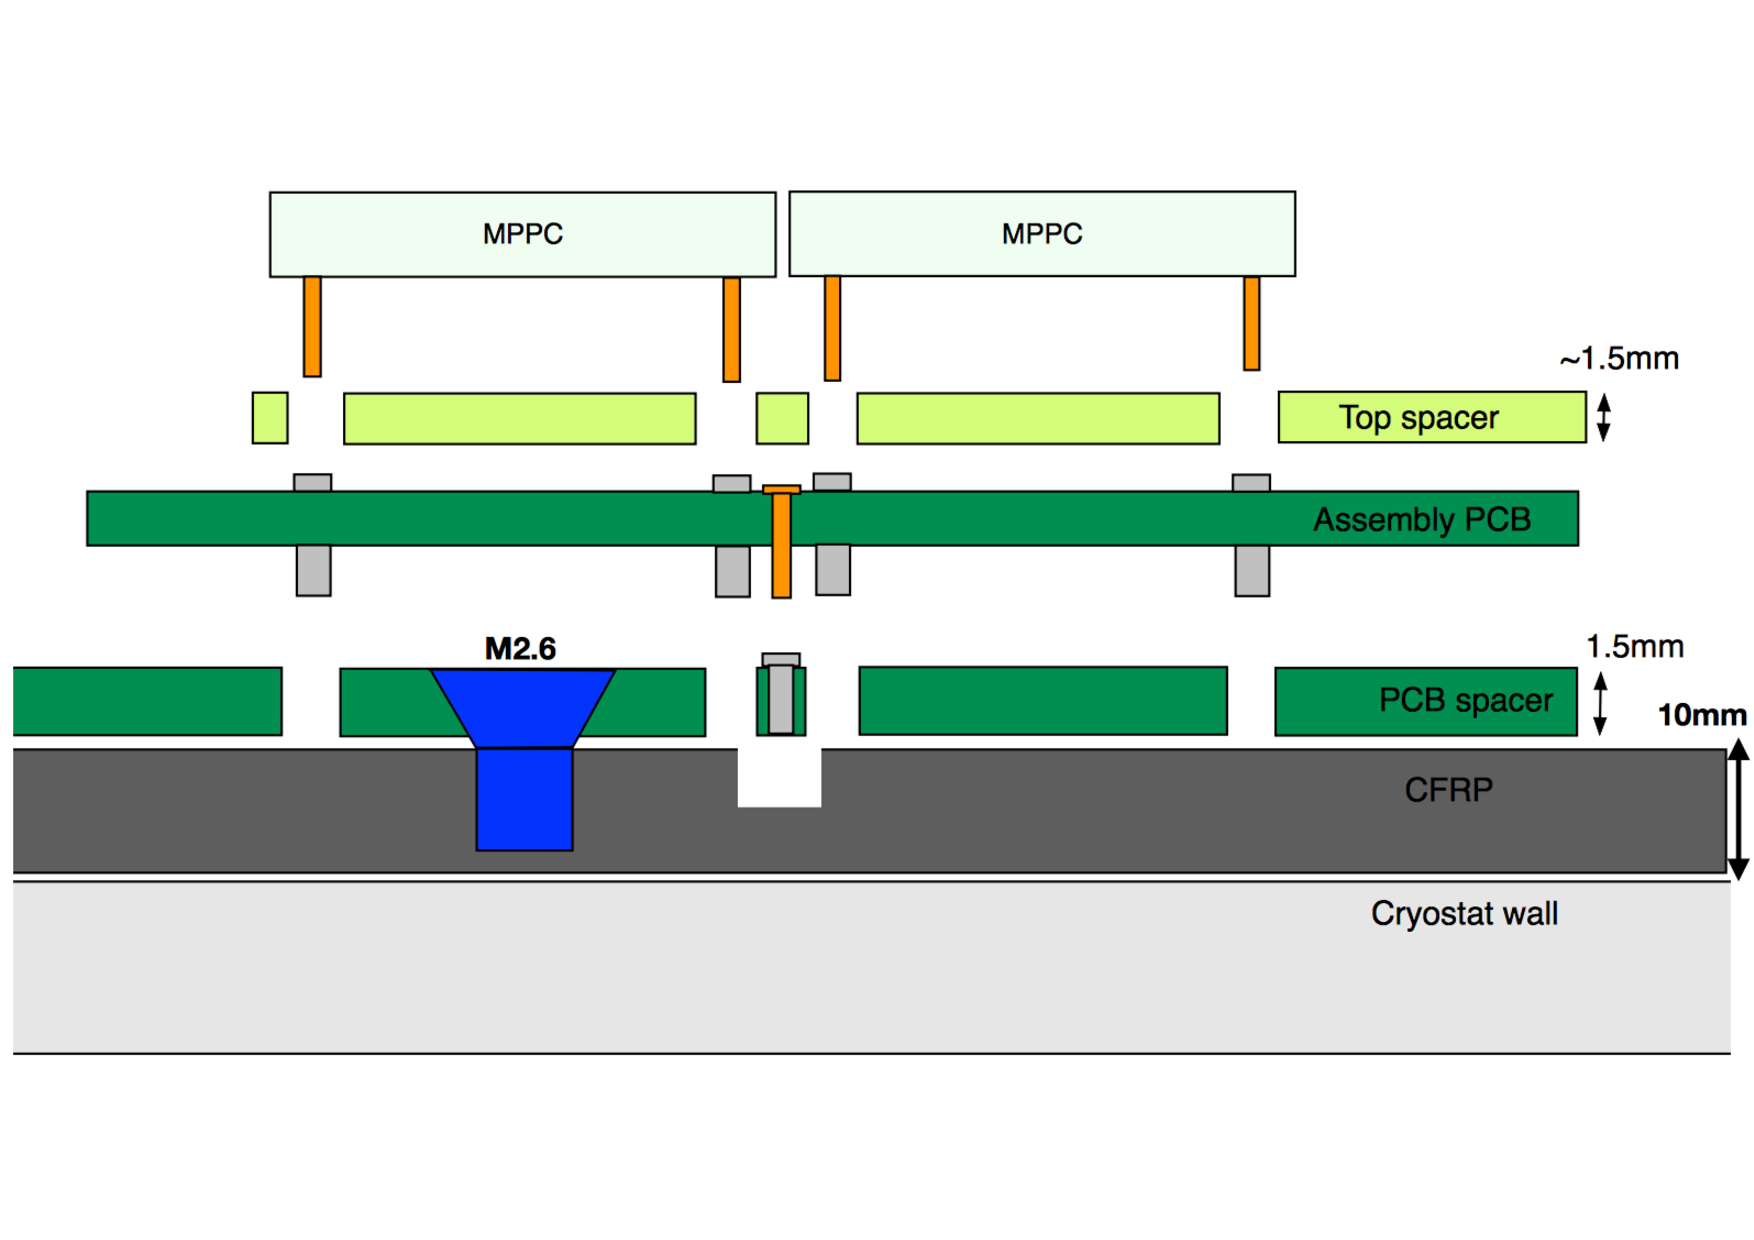
\includegraphics[width=4cm]{plots/MPPC_support.pdf}
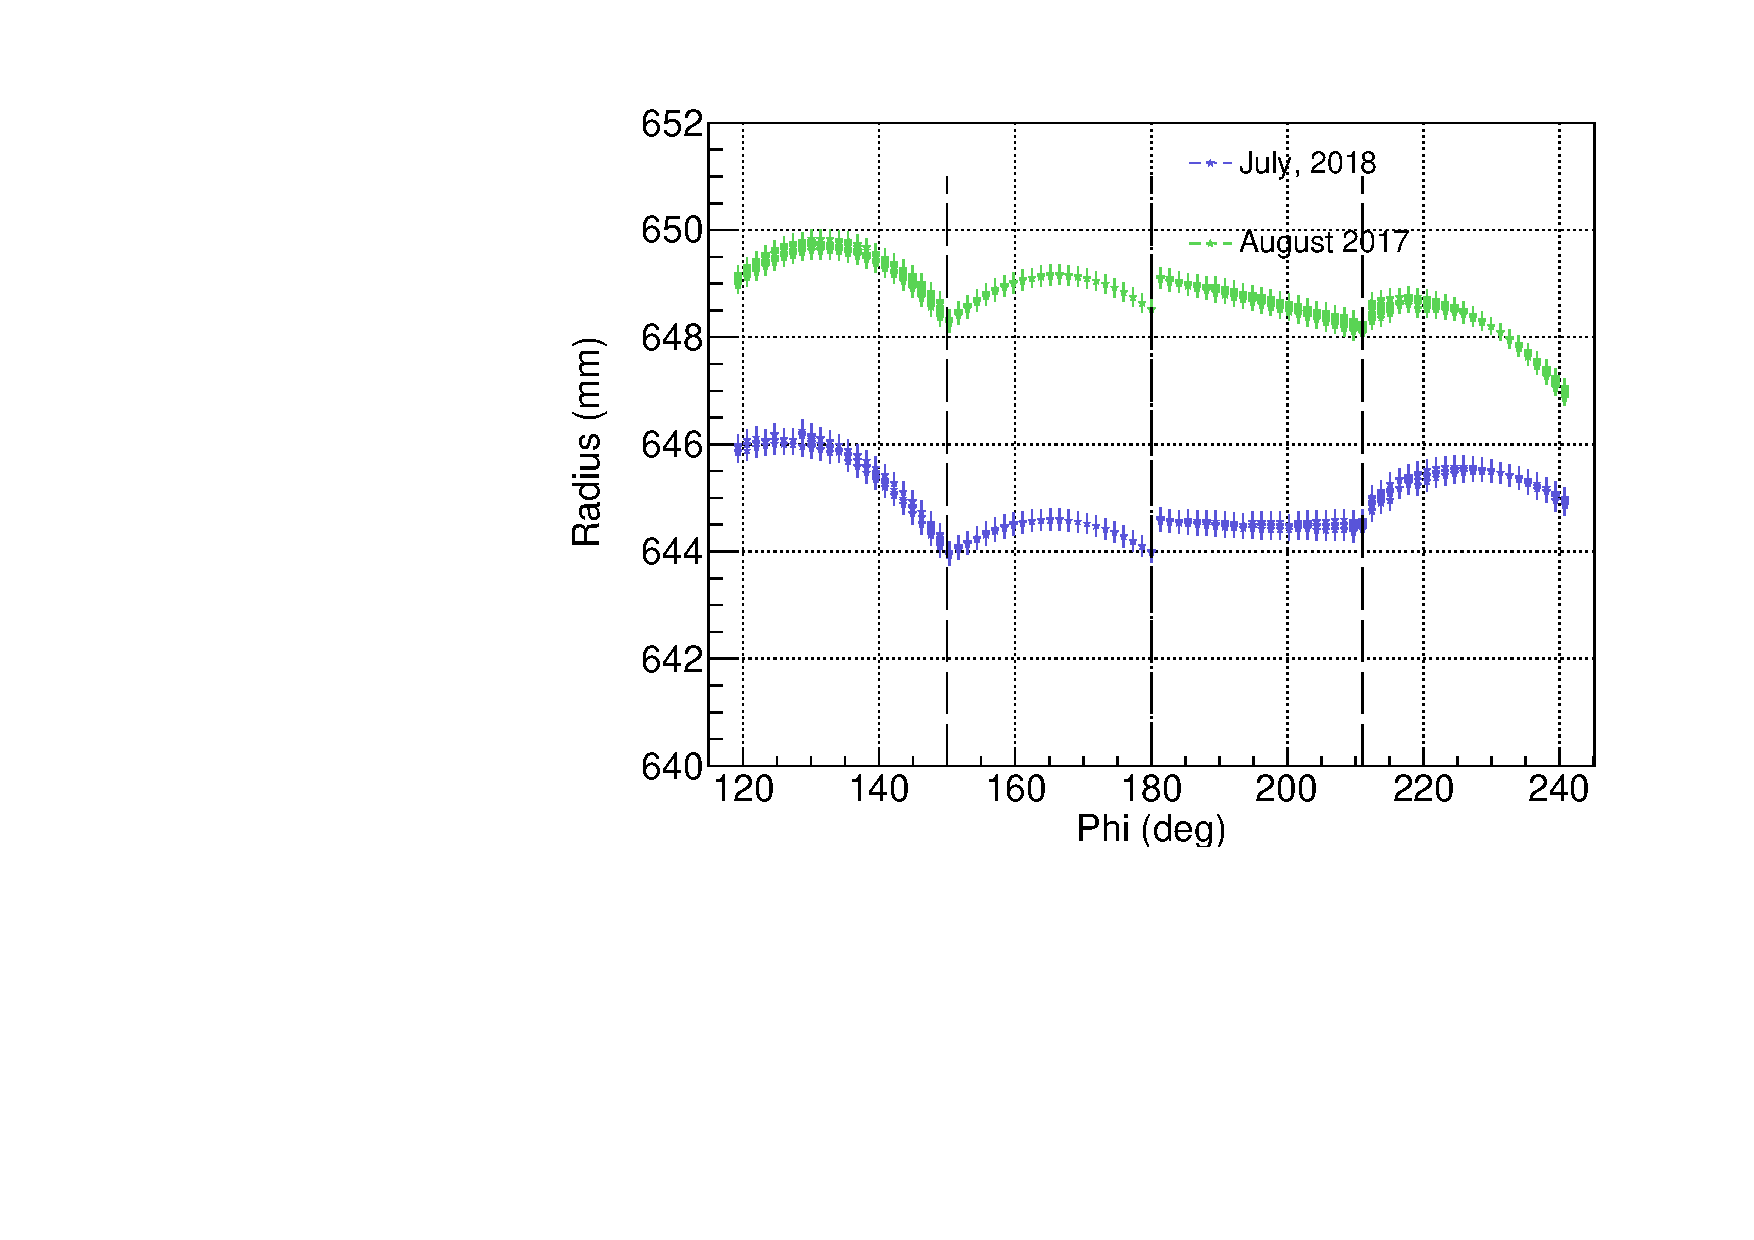
\includegraphics[width=4cm]{plots/2018/cRadius_1718}
\caption{ Radial coordinate of photodetectors with errors from 2017 and 2018
X-ray scans.  Black dashed lines indicate the edges of the CFRP plate.}
\label{fig:radiuscalculation} 
\end{center}
\end{figure}


